\documentclass[12pt,letterpaper]{scrartcl}
\usepackage[margin=1in]{geometry}
\usepackage{setspace}   % change spacing
\usepackage{times}  % Times New Roman
\usepackage[T1]{fontenc}    % Enable Type 1 font encoding (Cork Encoding)
\usepackage[english]{babel}     % Language settings
    %\renewcommand{\thesection}{\Roman{section}}

\usepackage{amsfonts,amssymb}
\usepackage[fleqn]{amsmath}
    \usepackage{mathtools}
\usepackage{graphicx}	% re-scale tree: \resizebox{}
\usepackage{framed,diagbox,fancybox}
\usepackage[usenames, dvipsnames,table]{xcolor}
\definecolor{shadecolor}{gray}{0.85}
\usepackage{enumitem}
\usepackage{makecell}	% alignment within tabular cell
    \renewcommand\theadalign{cl}

\usepackage[none]{hyphenat} % prevent LaTeX from hyphenating at the end of a line
\usepackage{comment}

\usepackage{pifont,fontawesome}

\usepackage{multirow,booktabs,hhline,makecell}  % format tabular cell
\usepackage{CJKutf8}    % input Chinese characters

\usepackage{caption}
\usepackage{slashbox}

% REFERENCES
\usepackage{csquotes} 
\usepackage[style=apa,
			natbib=true,
			backend=biber,
    		uniquename=false,
			doi=false,
			isbn=false,
			url=false,
			eprint=false]{biblatex}
    \AtEveryBibitem{%
      \clearfield{note}%
    }
\addbibresource{references.bib}
\renewcommand*{\nameyeardelim}{\space}  % Author Year \cite{}

\makeatletter
\renewrobustcmd*{\citet}{%
  \@ifstar
    {\AtNextCite{\AtEachCitekey{\let\ifciteseen\@firstoftwo}}%
     \textcite}
    {\textcite}}
\makeatletter

% SOME BASIC LINGUISTICS PACKAGES
\usepackage{tipa}
\usepackage{linguex}
\usepackage{tree-dvips}
\usepackage{semantic}
\usepackage{tikz-qtree}

% USER-DEFINED COMMANDS
\makeatletter
\newcommand*{\rom}[1]{\expandafter\@slowromancap\romannumeral #1@}
\makeatother    % number -> roman numeral

\newcommand{\ToneOne}[1] {\={#1}}
\newcommand{\ToneTwo}[1] {\'{#1}}
\newcommand{\ToneThree}[1] {\v{#1}}
\newcommand{\ToneFour}[1] {\`{#1}}

\title{How secondary cues contribute to tone identification}
%\subtitle{A case study of Mandarin Chinese}
\author{Agnes Bi}
\date{\today}

\begin{document}

\maketitle

%\begin{abstract}
%\noindent   \\
%
%\noindent  \textbf{Keywords}: tone, whisper, perceptual asymmetry, Mandarin Chinese
%\end{abstract}

\section{Motivation \& Questions}

It has long been established that fundamental frequency $F0$ serves as the primary cue to tone recognition (\cite{gandour1978PerceptionTone}, \cite{yip2002Tone}). Experimental studies have shown that even when all other cues are edited out of the auditory signals, native speakers of a tonal language can still reliably discriminate between various tones (\cite{fok1974perceptualstudytones}, \cite{abramson1978Staticdynamicacoustic}). A natural question to ask is then if the primary cue is taken away instead, can speakers differentiate tones with reasonable accuracy? In other words, is $F_0$ a necessary condition for tone classification? 

Whispered speech provides an ideal context for investigation. In whispers, fundamental frequency is absent since the periodic voicing is replaced by noise source, and, unlike synthetic stimuli, they are naturally occurring in daily conversations. This paper presents results from a pilot perception experiment, using Mandarin as a case study. The specific research questions of interest are:

	\begin{enumerate}[noitemsep]
		\item What is the overall accurate rate of tonal discrimination in whispers? 

		\item If it is significantly above chance, what are the secondary cues contributing to this process? 

		\item Do speakers show biases towards a certain tone?

	\end{enumerate}


\section{Background}

\subsection{Mandarin tones basics}

Mandarin Chinese has four contrastive lexical tones: Tone 1 (high level 55), Tone 2 (rising 35), Tone 3 (low falling rising 214), and Tone 4 (falling 51). In citation forms of normal speech, Tone 3 has the longest duration and lowest average intensity, while Tone 4 has the shortest duration and highest average intensity (\cite{chang.yao2007ToneProductionWhispered}). The typical patterns of the four tones in citation form are illustrated in the figure below, where each tone is plotted with their average duration proporation to the average duration of Tone 3 (\cite{liu.samuel2004PerceptionMandarinLexical}, adapted from \cite{xu1997Contextualtonalvariationsa}):

%TODO: Add an illustration of the tonal space
	\begin{figure}[h]
		\centering
		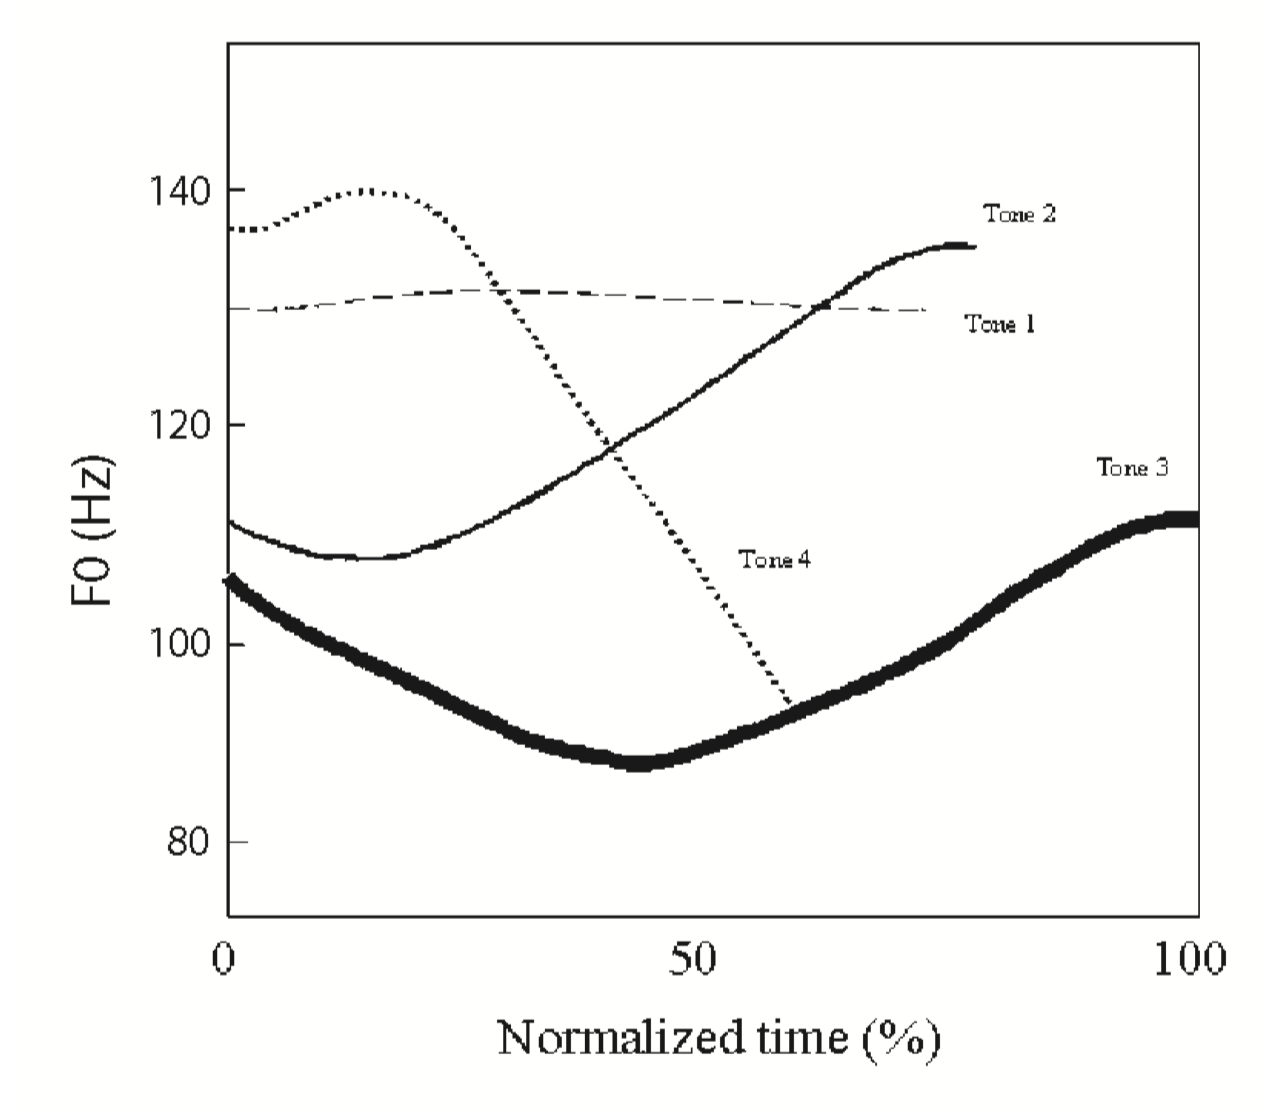
\includegraphics[scale=0.45]{F0_contours}
		\caption{Typical $F0$ contours for the four contrastive tones in Mandarin}
	\end{figure}

\subsection{Previous studies}

%Suppose people can, in fact, distinguish various tones to some extent in whispers, the main point of contention then becomes: is it largely thanks to the speaker intentionally augmenting secondary cues such as duration and intensity envelope, or is it because in the absence of F0, listeners are more sensitive or pay more attention to these cues? The former is the \textsc{production enhancement} hypothesis, supported by studies such as \cite{liu.samuel2004PerceptionMandarinLexical}, and the latter is the \textsc{perceptual compensation} hypothesis, advocated by \cite{jiao.xu2019WhisperedMandarinhas} among others. 

Previous perception studies show a range of accuracy rates of tone perception in whispered speech: some studies have reported performance slightly higher than chance (\cite{abramson1972TonalExperimentsWhispered} on Thai; \cite{miller1961WordToneRecognition} on Vietnamese), and in a few cases, well above chance (\cite{jensen1958RecognitionWordTones} on Norwegian, Swedish, Slovenian, and Mandarin). There are two potential reasons for this discrepancy in the literature: (1) early studies have varying scope of data and often do not examine the full paradigms; (2) for the statistical analysis part, only \textit{percent correct} is used for evaluating whether the identification is successful, which fails to isolate potential bias.

\cite{liu.samuel2004PerceptionMandarinLexical} is one of the first comprehensive experiments

On a related note, neural network models trained without explicit $F_0$ information manually encoded, such as the ones tested in \cite{ryant.etal2014Highlyaccuratemandarin} and in \cite{chen.etal2016ToneClassificationMandarina}, perform remarkably well in tone classification for phonated speech. This may suggest that some non-$F_0$ phonetic dimensions are jointly utilized by the models to predict tonal category.

The main goal of this project is to directly probe the two secondary cues, namely \textit{duration} and \textit{temporal envelope}, that have been shown to vary with lexical tones (\cite{tseng1981AcousticPhoneticStudy}, \cite{fu.zeng2000Identificationtemporalenvelope}, \cite{kong.zeng2006Temporalspectralcues}, a.o.).

\section{Methods}

The present study is a slightly simplified replicate of a perception experiments presented in \cite{jiao.xu2019WhisperedMandarinhas} (J\&X). Unlike J\&X, we did not test intonation as a dimension of variable. 

\subsection{Stimuli}

The perception stimuli are five sets of monosyllables composed of only vowels (/\textipa{7}/ and /u/), with glide onsets (/i/-[ji] and /y/-/[jy]) or with nasal onset (/\textipa{a}/-\textipa{ma}). They are the same stimuli as the ones used in J\&X except the /a/ quadruplet, since syllables composed of only /a/ are generally discourse markers with meanings such as `ah' or `what?' and they correspond to the same character, which makes it difficult to indicate in the forced-choice task. The five sets of tone quadruplets are shown in Table 1.

\vspace{0.25cm}
\begin{center}
\begin{CJK*}{UTF8}{gkai}
    \begin{tabular}{|l|l|c|c|c|c|c|}
        \hline
        \multicolumn{2}{|l|}{\diaghead{\theadfont Diag Columnmnmn}%
        {Tone}{Vowel}} & /\textipa{ma}/ & /\textipa{7}/ & /\textipa{i}/ & /\textipa{u}/ & /\textipa{y}/ \\ \hhline{|=|=|=|=|=|=|=|}
        \multirow{3}{*}{T1} & Character & 妈 & 婀 & 衣 & 乌 & 迂 \\ \cline{2-7} 
         & Pinyin & m\={a} & \={e} & y\={\i} & w\={u} & y\={u} \\ \cline{2-7} 
         & Glossary & `mother' & `graceful' & `clothes' & `black' & `winding' \\ \hhline{|=|=|=|=|=|=|=|}
         \multirow{3}{*}{T2} & Character & 麻 & 鹅 & 姨 & 无 & 鱼 \\ \cline{2-7} 
         & Pinyin & m\'{a} & \'{e} & y\'{\i} & w\'{u} & y\'{u} \\ \cline{2-7} 
         & Glossary & `hemp' & `goose' & `aunt' & `nothing' & `fish' \\ \hhline{|=|=|=|=|=|=|=|}
         \multirow{3}{*}{T3} & Character & 马 & 恶 & 椅 & 五 & 雨 \\ \cline{2-7} 
         & Pinyin & m\v{a} & \v{e} & y\v{\i} & w\v{u} & y\v{u} \\ \cline{2-7} 
         & Glossary & `horse' & `nausea' & `chair' & `five' & `rain'  \\ \hhline{|=|=|=|=|=|=|=|}
         \multirow{3}{*}{T4} & Character & 骂 & 饿 & 意 & 物 & 玉 \\ \cline{2-7} 
         & Pinyin & m\`{a} & \`{e} & y\`{\i} & w\`{u} & y\`{u} \\ \cline{2-7} 
         & Glossary & `scold' & `hungry' & `meaning' & `thing' & `jade' \\ \hline
    \end{tabular}
\end{CJK*}
\captionof{table}{Target Stimuli}\label{stimuli}
\end{center}
\vspace{0.25cm}

The stimuli are recorded by two female native speakers of Mandarin, who grew up in eastern coastal China. Speakers read through the same word list in different randomized order. For each speaker, 5 (syllables) * 4 (tones) * 2 (speech types) * 2 (repetition) = 80 stimuli are recorded. Speakers are instructed to read through the list alternating between normal speech and whisper for each token. The phonated version is read first in the first repetition, and whispered first in the second repetition.
 
The recordings are made  in a sound-proof booth at a sampling rate of 44.1kHz as 16-bit format mono sound files.


\subsection{Participants}

Four native Mandarin speakers between the age of 22-27 participated in the perception experiment, among which two are females and two are males.\footnote{Data from another female speaker was collected but not included in the subsequent statistical analysis, as her dominant language is Cantonese, instead of Mandarin.} None of the participants reported any hearing or speech impairment.

\subsection{Procedure}

The written instructions were given in English, but explained again in Mandarin prior to the practice trials. After a stimulus is played, participants are given four options, each is a simplified Chinese character corresponding to one of the relevant tone quadruplets. They were told to choose the closest character to what they heard. Each audio can be repeated at most once. This is to avoid the situation when the participant got distracted and accidentally missed the word. Participants are encouraged to take a break halfway through the experiment. The entire study lasts approximately 15 minutes.

\section{Analyses}

\subsection{Data pruning}

A total of 596 observations, excluding practice trials, are collected. The reaction time data in seconds look as follows:

\begin{center}
    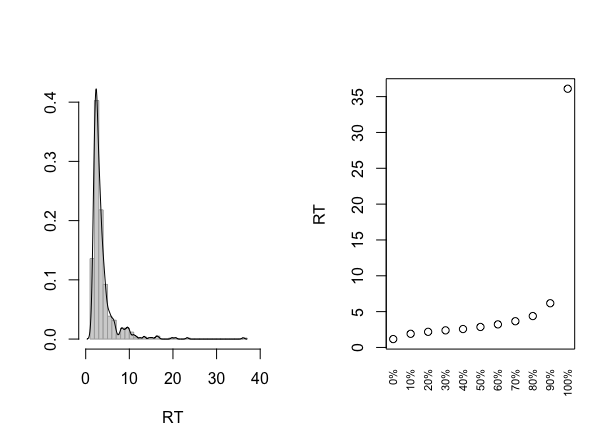
\includegraphics[scale=0.45]{data_pruning}
    \captionof{figure}{Distribution of reaction time data}\label{RT}
\end{center}

95\% of the data points fall between 1.17s and 9.11s. Since there are some extreme outliers, the observations with RT greater than 10s are discarded, which is about 3.5\% of the data.

\subsection{Accuracy \& confusion matrix}

As expected, tones are generally much worse identified in whispered than in phonated utterances (55.5\% vs. 99.4\%). In phonated utterances, all tones were perceived essentially at ceiling. In whispers, the picture is more complicated.  The identification rate drops to almost chance level for T1 (29.6\%) and T2 (24.2\%), but much less for T4 (61.5\%), which is consistent with the findings in J\&X (23.86\%, 31.06\%, and 60.23\%, respectively). However, at least on the surface, T3 identification is, surprisingly, still near ceiling at 94.7\% (cf. 84.47\% in J\&X).

\begin{figure}[h]
	\begin{minipage}{0.45\textwidth}
	\begin{center}
		\begin{tabular}{|c|c|c|c|c|}
			\hline
			\backslashbox{{\scriptsize Produced}}{{\scriptsize Perceived}}  & 1 & 2 & 3 & 4 \\ \hline
			T1 & \cellcolor[HTML]{FFFFC7}16 & 7 & 12 & 19 \\ \hline
			T2 & 8 & \cellcolor[HTML]{FFFFC7}15 & 32 & 7 \\ \hline
			T3 & 1 & 2 & \cellcolor[HTML]{FFFFC7}71 & 1 \\ \hline
			T4 & 10 & 4 & 11 & \cellcolor[HTML]{FFFFC7}40 \\ \hline
		\end{tabular}
	\end{center}
	\end{minipage}
	\begin{minipage}{0.55\textwidth}
	\begin{center}
		\begin{tabular}{|c|c|c|c|c|}
			\hline
			\backslashbox{{\scriptsize Produced}}{{\scriptsize Perceived}} & 1 & 2 & 3 & 4 \\ \hline
			T1 & \cellcolor[HTML]{FFFFC7}29.6\% & 13.0\% & 22.2\% & 35.2\% \\ \hline
			T2 & 12.9\% & \cellcolor[HTML]{FFFFC7}24.2\% & 51.6\% & 11.3\% \\ \hline
			T3 & 1.3\% & 2.7\% & \cellcolor[HTML]{FFFFC7}94.7\% & 1.3\% \\ \hline
			T4 & 15.4\% & 6.2\% & 16.9\% & \cellcolor[HTML]{FFFFC7}61.5\% \\ \hline
		\end{tabular}
	\end{center}
	\end{minipage}
\captionof{table}{Aggregated confusion matrix in whispered speech}\label{Conf}
\end{figure}

The pattern of confusion in tone recognition is quite interesting in itself, and can potentially provide some insights into how the four tones occupy the abstract tonal space. When Tone 1 stimuli were presented, listeners more often identified it as Tone 4 than itself.  Strikingly, Tone 2 is identified much more often as Tone 3 than itself, but Tone 3 is rarely misidentified as Tone 2. The overwhelming bias toward Tone 3 is not observed in either \cite{liu.samuel2004PerceptionMandarinLexical} or \cite{jiao.xu2019WhisperedMandarinhas}. In the next subsection, I will venture a guess to the cause of this disparity.

\subsubsection{Possibly, partition of speakers?}

I would like to state upfront that what the results in this section might suggest cannot be taken at face value considering the small sample size. 

By fitting a binomial logistic regression model with accuracy rate as dependent variable and speech type, tone, participant gender, stimulus duration as independent variables (C = 0.942), we find that participant gender is a statistically significant predictor of accuracy rate (with gender = female being the reference level, b = -0.7168, SE = 0.3085, p = 0.0201 < 0.05), which seems quite puzzling. I hypothesize that there are two distinct classes of speakers in terms of how they deal with ``confusing'' tones in whispers, Tone 1 and Tone 2 in particular, and it just happens to be the case that in this particular experiment, the two natural classes coincide with gender divide. Class \rom{1} listeners are equally likely to judge Tone 1 as Tone 1 or Tone 4, and to judge Tone 2 as Tone 2 or Tone 4. The pattern would be similar to what's shown in Table 5:

%\vspace{0.25cm}
%\begin{minipage}{0.5\textwidth}
%\begin{center}
%	\begin{tabular}{l|l|l}
%		 & incorrect & correct  \\ \hline
%        phonated & 1 & 159  \\ \hline
%        whispered & 49 & 80 
%	\end{tabular}
%\end{center}
%\end{minipage}
%\begin{minipage}{0.5\textwidth}
% \begin{center}
%	\begin{tabular}{l|l|l}
% 		& incorrect & correct  \\ \hline
%		phonated & 0.6\% & 99.4\%  \\ \hline
%		whispered & 38\% & \cellcolor[HTML]{FFFFC7}62\%
%	\end{tabular}
%\end{center}
%\end{minipage}
%\captionof{table}{Accuracy rate of female participants in phonated versus whispered speech}
%\vspace{0.25cm}

\begin{figure}
	\begin{minipage}{0.45\textwidth}
	\begin{center}
		\begin{tabular}{|c|c|c|c|c|}
			\hline
			\backslashbox{{\scriptsize Produced}}{{\scriptsize Perceived}}  & 1 & 2 & 3 & 4 \\ \hline
			T1 & \cellcolor[HTML]{FFFFC7}10 & 4 & 5 & \cellcolor[HTML]{FFFFC7}9 \\ \hline
			T2 & 3 & \cellcolor[HTML]{FFFFC7}12 & \cellcolor[HTML]{FFFFC7}10 & 4 \\ \hline
			T3 & 1 & 2 & 34 & 1 \\ \hline
			T4 & 2 & 2 & 6 & 24 \\ \hline
		\end{tabular}
	\end{center}
	\end{minipage}
	\begin{minipage}{0.55\textwidth}
	\begin{center}
		\begin{tabular}{|c|c|c|c|c|}
			\hline
			\backslashbox{{\scriptsize Produced}}{{\scriptsize Perceived}} & 1 & 2 & 3 & 4 \\ \hline
			T1 & \cellcolor[HTML]{FFFFC7}35.7\% & 14.3\% & 17.9\% & \cellcolor[HTML]{FFFFC7}32.1\% \\ \hline
			T2 & 10.3\% & \cellcolor[HTML]{FFFFC7}41.4\% & \cellcolor[HTML]{FFFFC7}34.5\% & 13.8\% \\ \hline
			T3 & 2.6\% & 5.3\% & 89.5\% & 2.6\% \\ \hline
			T4 & 5.9\% & 5.9\% & 17.6\% & 70.6\% \\ \hline
		\end{tabular}
	\end{center}
	\end{minipage}
\captionof{table}{Confusion matrix in whispered speech of female participants}
\end{figure}

Class \rom{2} listeners are more inclined to default to Tone 3 or Tone 4, when presented with Tone 2 or Tone 1 stimuli in whispers. The pattern in Table 6 falls along this line:

%\vspace{0.25cm}
%\begin{minipage}{0.5\textwidth}
%\begin{center}
%	\begin{tabular}{l|l|l}
%		 & incorrect & correct  \\ \hline
%        phonated & 1 & 158  \\ \hline
%        whispered & 65 & 62 
%	\end{tabular}
%\end{center}
%\end{minipage}
%\begin{minipage}{0.5\textwidth}
% \begin{center}
%	\begin{tabular}{l|l|l}
% 		& incorrect & correct  \\ \hline
%		phonated & 0.6\% & 99.4\%  \\ \hline
%		whispered & 51.2\% & \cellcolor[HTML]{FFFFC7}48.8\%
%	\end{tabular}
%\end{center}
%\end{minipage}
%\captionof{table}{Accuracy rate of male participants in phonated versus whispered speech}
%\vspace{0.25cm}

\begin{figure}
	\begin{minipage}{0.45\textwidth}
	\begin{center}
		\begin{tabular}{|c|c|c|c|c|}
			\hline
			\backslashbox{{\scriptsize Produced}}{{\scriptsize Perceived}}  & 1 & 2 & 3 & 4 \\ \hline
			T1 & \cellcolor[HTML]{FFFFC7}6 & 3 & 7 & \cellcolor[HTML]{FFFFC7}10 \\ \hline
			T2 & 5 & \cellcolor[HTML]{FFFFC7}3 & \cellcolor[HTML]{FFFFC7}22 & 3 \\ \hline
			T3 & 0 & 0 & 37 & 0 \\ \hline
			T4 & 8 & 2 & 5 & 16 \\ \hline
		\end{tabular}
	\end{center}
	\end{minipage}
	\begin{minipage}{0.55\textwidth}
	\begin{center}
		\begin{tabular}{|c|c|c|c|c|}
			\hline
			\backslashbox{{\scriptsize Produced}}{{\scriptsize Perceived}} & 1 & 2 & 3 & 4 \\ \hline
			T1 & \cellcolor[HTML]{FFFFC7}23.1\% & 11.5\% & 26.9\% & \cellcolor[HTML]{FFFFC7}38.5\% \\ \hline
			T2 & 15.2\% & \cellcolor[HTML]{FFFFC7}9.1\% & \cellcolor[HTML]{FFFFC7}66.7\% & 9.1\% \\ \hline
			T3 & 0\% & 0\% & 100\% & 0\% \\ \hline
			T4 & 25.8\% & 6.5\% & 16.1\% & 51.6\% \\ \hline
		\end{tabular}
	\end{center}
	\end{minipage}
\captionof{table}{Confusion matrix in whispered speech of male participants}
\end{figure}

Further studies drawn from a much larger sample size are needed to test this hypothesis. If it does have some empirical ground, we could argue for some intrinsic connection between Tone 1 and Tone 4, and between Tone 2 and Tone 3 that make them pair-wise more easily confusable.


\subsection{Perceptual bias and distances}

As expected, tone identification is much less accurate in whispered than in phonated utterances (55.5\% vs. 99.4\%). In phonated utterances, all tones were perceived essentially at ceiling. In whispers, the picture is more complicated. The identification rate drops to almost chance level for T1 (29.6\%) and T2 (24.2\%), but less so for T4 (61.5\%), which is consistent with the findings in J\&X (23.86\%, 31.06\%, and 60.23\%, respectively). However, at least on the surface, T3 identification is, surprisingly, still near ceiling at 94.7\% (cf. 84.47\% in J\&X). 


However, the high accuracy rate in identifying T3 should not be taken at face value, since it is likely due to a bias defaulting to T3 when the participant is uncertain. A Biased Choice loglinear model, with the baseline for response set at T3, is fitted to test this hypothesis. 

\begin{comment}
Call:
glm(formula = value ~ stimulus + response + d, family = poisson(link = "log"), 
    data = agg_confmat)
    
Coefficients:
             Estimate Std. Error z value Pr(>|z|)    
(Intercept)  4.881961   0.320560  15.229  < 2e-16 ***
stimulus2    0.001343   0.269116   0.005   0.9960    
stimulus3   -0.619281   0.320560  -1.932   0.0534 .  
stimulus4    0.171290   0.225269   0.760   0.4470    
response1   -2.109372   0.320560  -6.580 4.70e-11 ***
response2   -2.175254   0.310871  -6.997 2.61e-12 ***
response4   -1.364372   0.304419  -4.482 7.40e-06 ***
d1.2        -0.725981   0.314648  -2.307   0.0210 *  
d1.3        -2.380275   0.400544  -5.943 2.81e-09 ***
d1.4        -0.597176   0.242093  -2.467   0.0136 *  
d2.3        -1.416213   0.330858  -4.280 1.87e-05 ***
d2.4        -1.544211   0.343653  -4.494 7.01e-06 ***
d3.4        -2.678014   0.380970  -7.029 2.07e-12 ***
---
Signif. codes:  0 ‘***’ 0.001 ‘**’ 0.01 ‘*’ 0.05 ‘.’ 0.1 ‘ ’ 1
\end{comment}

From the output above, we can estimate bias parameters for each tone, and calculate estimated perceptual distance between each pair of tones. 

Let's first calculate the bias parameters. Since all three response coefficients have $p \ll  0.05$, we can safely conclude that the bias towards T1, T2, and T4 are significantly different from that towards T3. Normalizing the $e^\lambda$ values gives us the BCM bias parameters.

\vspace{0.25cm}
\begin{center}
    \begin{tabular}{c|p{4cm} p{4cm} p{4cm}}
        {} & loglinear coefficient $\lambda$ & $e^\lambda$ & bias parameter b \\ \hline
        T1 & -2.109372 & 0.12131412778 & 0.0814 \\
        T2 & -2.175254 & 0.11357930086 & 0.0762 \\
        T3 & 0 & 1 & 0.6709 \\
        T4 & -1.364372 & 0.25554110542 & 0.1715
    \end{tabular}
    \captionof{table}{Bias parameters calculation}
\end{center}
\vspace{0.25cm}

There is an overwhelming bias towards T3, which was not noted in either \cite{liu.samuel2004PerceptionMandarinLexical} or \cite{jiao.xu2019WhisperedMandarinhas}. 

Although $d$ values obtained in BCM are not quite ``distances" in the usual sense, it is interesting to note that even in whispered speech, each pair of tones are still distinct enough (all 6 pairs with $p < 0.05$) from each other. Specifically, $D_{\text{T1T2}} = 0.725981$, $D_{\text{T1T3}} = 2.380275$, $D_{\text{T1T4}} = 0.597176$, $D_{\text{T2T3}} = 1.416213$, $D_{\text{T2T4}} = 1.544211$, $D_{\text{T3T4}} = 2.678014$, with T3 and T4 being most distinct from each other and T1 and T4 the least. 

A closer look into each participant's data seems to suggest a difference in bias. Hence, participant is added as an additional variable in BCM to test the effects. Unfortunately, given the limited data, 3 coefficients are not defined because of singularities.

In sum, BCM reveals a strong bias towards T3, but tones in whispered speech are still perceptually distinct. This encourages further investigation into what, then, are the cues speakers rely on for tone identification when $F_0$ is taken away. The two obvious candidates are duration and amplitude, and I will explore the former in the next subsection.




\subsection{Reaction Time}

\begin{center}
	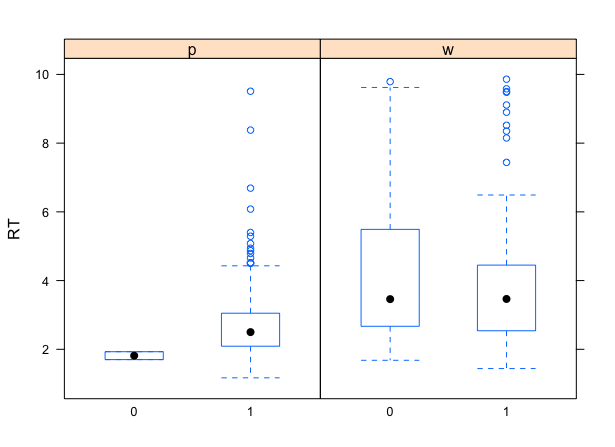
\includegraphics[scale=0.45]{RT}
	\captionof{figure}{Reaction time distribution given accuracy of the response}
\end{center}

It does not come as a surprise that in general, the reaction time for whispered speech is significant longer than the RT for phonated speech. It is worth noting that based on the short RT for the two misidentified phonated tokens, the mistakes are most likely due to technical error such as pressing the wrong key than genuine confusion.


\subsection{Duration}

Many studies have suggested temporal envelope and intensity being possible cues for tone recognition in whispers. \cite{liu.samuel2004PerceptionMandarinLexical} find a correlation between syllable duration and tone perception. This subsection presents some preliminary results as I try to look into the correlation between accuracy rate and duration of the stimuli.

The duration data used here are audio clip length extracted automatically using a python script. The recordings were not quite segmented based on a consistent criterion, since the beginning and ending of a whispered sound is oftentimes difficult to tell on the spectrogram. Due to time limitation, I was not able to go back to the original recordings and measure duration of each token manually, but that will be the next step for this project.

A box and whisker plot is given below; 0 means incorrect response, and the y-axis is the duration of the corresponding set of stimuli in seconds.

%\begin{center}
%	\includegraphics[scale=0.5]{Duration}
%\end{center}

An ANOVA test is performed to determine whether leaving the variable Duration out of the binomial logistic regression model would significantly reduce the deviance. Duration is not shown to be a significant predictor of accuracy rate ($p = 0.4279 \gg 0.05$).


\section{Analysis}


\subsection{Duration}

Many studies have suggested temporal envelope and intensity being possible cues for tone recognition in whispers. \cite{liu.samuel2004PerceptionMandarinLexical} find a correlation between syllable duration and tone perception. This subsection presents some preliminary results as I look into the correlation between response and duration\footnote{The duration data used here are audio clip length extracted automatically using a python script. The recordings were not quite segmented based on a consistent criterion, since the beginning and ending of a whispered sound is oftentimes difficult to pinpoint on the spectrogram. A better approach would be to measure each token duration manually.} of the stimuli.

Let's hypothesize that a longer duration should result in participants favoring T3 and disfavoring T4. A multinomial logistic regression is used to model the decision process, with stimuli and duration as predictors.

\begin{comment}
Call:
multinom(formula = response ~ stimulus * RT, data = ws)

Coefficients:
  (Intercept)  stimulus2 stimulus3  stimulus4          RT stimulus2:RT stimulus3:RT
1   0.6233646 -2.8019236 -8.662911 -0.7433690 -0.07859640    0.2863913    0.8825459
2  -1.2063596 -0.5910529 -3.626705 -0.5149423  0.14118120    0.1258540    0.2030838
4   0.2725518 -3.5089639 -3.794896  0.8427763  0.04151562    0.3740646   -0.2829901
  stimulus4:RT
1  0.083976064
2  0.002461432
4 -0.003859209

Std. Errors:
  (Intercept) stimulus2 stimulus3 stimulus4        RT stimulus2:RT stimulus3:RT
1   0.9291642  1.392299  3.121081  1.387779 0.1976337    0.3132259    0.4773149
2   1.1728868  1.439296  2.070210  1.826018 0.2233693    0.2964322    0.4358926
4   0.8941857  1.419476  2.999283  1.202058 0.1816308    0.2930758    0.9404803
  stimulus4:RT
1    0.2836323
2    0.3346118
4    0.2405578

Residual Deviance: 459.1403 
AIC: 507.1403

\end{comment}

I'm not quite sure how to interpret the results of a multinomial logistic regression, but a model with only stimulus type as the predictor seems to give a better fit (lower AIC), which contradicts our intuition.

\begin{comment}
Call:
multinom(formula = response ~ stimulus, data = ws)

Coefficients:
  (Intercept)  stimulus2 stimulus3  stimulus4
1   0.2876653 -1.6739426 -4.550332 -0.3829851
2  -0.5390443 -0.2185998 -3.030547 -0.4725561
4   0.4594601 -1.9792723 -4.722072  0.8315423

Std. Errors:
  (Intercept) stimulus2 stimulus3 stimulus4
1   0.3818757 0.5496172 1.0769864 0.5802939
2   0.4755934 0.5693016 0.8604085 0.7530613
4   0.3687326 0.5568405 1.0723709 0.5018700

Residual Deviance: 468.7348 
AIC: 492.7348 

\end{comment}

\section{Discussion}

To summarize, Tone 3 and Tone 4 overall show significantly above chance identification rates in whispers, with the former near ceiling. Tone 1 and Tone 2 identification are essentially at chance.

In whispered speech, participants show a strong bias towards Tone 3 and a weak one towards Tone 4. However, the four tones seem to still be perceptually distinct from each other, the reason of which remains unclear.

Two interesting perceptual asymmetries are observed: (a) Tone 2 is much more frequently misidentified as Tone 3 than Tone 3 as Tone 2; and (b) Tone 1 is  more often misidentified as Tone 4 than Tone 4 as Tone 1. The similarity between Tone 2 and Tone 3 has been argued for extensively in literature (\cite{shen1989ProsodyMandarinChinese}, \cite{liu.samuel2004PerceptionMandarinLexical}, a.o.), but the connections between Tone 1 and Tone 4 need further investigation. An obvious one is that both Tone 1 (55) and Tone 4 (51) have high pitch register onsets. Since amplitude contour mirrors F0 contour (\cite{whalen.xu1992InformationMandarintones}), one could argue that onset amplitude is an important cue to tone identification in whispers, as it first bipartitions logical space to either choosing between Tone 1 and Tone 4 if the onset amplitude is high, or choosing between Tone 2 and Tone 3 if the onset amplitude is low. The confusion between Tone 1 and Tone 4 and between Tone 2 and Tone 3 seem to suggest that listeners are less sensitive to the overall shape of the amplitude contour. Moreover, assuming complex contour tones (Tone 3) are structurally more complicated than simple contour tones (Tone 2, Tone 4), and in turn, more complicated than level tones (Tone 1), when there is insufficient information regarding the overall shape of the amplitude contour or when listeners cannot determine it for certain, at least a subset of the listeners defaults to the more complicated structure (hypothesized Class \rom{2} speakers in section IV.2.1).

\subsection{Potential Confounds}

To end this squib, I will point out some potential confounds of the present study and what I have learned from this pilot experiment.

First of all, all the response options given in each trial are characters corresponding to minimal tone quadruplets, which could make research objective quite transparent to the participants. This is a drawback in the experimental design, and in future experiments, I should incorporate response options with, for example, varying syllables as filler items.

Secondly, since the audio clips are recorded separately by two different speakers, the average amplitude within each speech type should be normalized across speakers.\footnote{Even though there was not a main effect of Speaker in the findings here, it is probably in general a good practice to control individual variation.}

Thirdly, it is nontrivial to establish a consistent segmenting criterion for the whispered tokens, as their left and right boundaries are often fuzzy. Directly comparing acoustic properties of whispered syllables with their phonated counterparts can be tricky. In the present study, the boundaries of a whispered sound are largely determined by its spectrogram shape, and when there are clear formants, they seem to be consistent with the phonated version. Note in many cases, Praat cannot generate reliable formant readings (for f1 in particular), which suggests that automated data extraction is likely to fail. % "seems unreliable at best" -- Peter 

%%%%%%%%%%%%%%%%%%%%%%%%%%%%%%%%%%%%%%%%%%%%%%%%%%%%%%%%%%%%%%
\newpage
\printbibliography

\end{document}

